\subsubsection{Exercise}

Since $G_d(s) = \frac{10}{s+1}$, the cross-over frequency is $w_c = 10$ rad/s.

We have the following result:

$$\forall \omega < \omega_c, |Gd(j\omega)| >1$$

Control action is needed at least for $\omega \in [0,\omega_c]$.

Here, we will try to design $F_y$ in such a way that:
$$L(s) = F_y G = \frac{\omega_c}{s}$$

Let:
$$F_y = G^{-1} \frac{\omega_c}{s} = \frac{200 s^3 + 4200 s^2 + 84000 s + 80000}{160000 s}$$

This controller has $3$ zero and $1$ pole. Thus, it is not proper. However -- using \texttt{Matlab} -- we can plot the step response of the system and the step response to a step perturbation (see Figure \ref{stepNonProper}).

\begin{figure}[h!t]
    \centering
    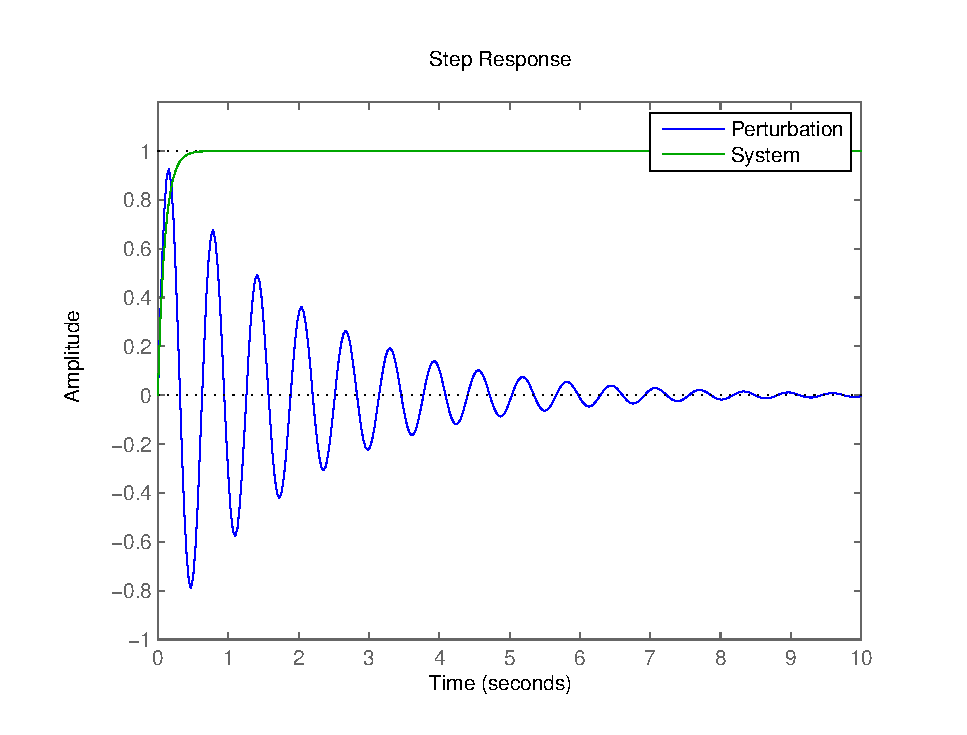
\includegraphics[width=\linewidth]{fig/stepNonProper421.eps}
    \caption{Non-proper step response of the system}
    \label{stepNonProper}
\end{figure}

We can see that even if the performance are poor (Error static $\leq 5\%$ for $t \geq t_d = 7$ s) we still have an attenuation of the perturbation and a step response of good quality.

Assuming that this controller is the one we want to implement, we need to design it in a proper way. For now, it has $3$ zeros and $1$ pole. Therefore it is needed to add two more poles.

Let:
$$F_y(s) = G^{-1}\frac{\omega_c}{s(s+p_1)(s+p_2)}$$

We need to choose $p_{1,2}$ in order to not change the system performance two much.

We use the following criteria:

\begin{itemize}
    \item $p_1 = p_2$
    \item $p_1$ and $p_2$ take action after $\omega_c$ 
\end{itemize}

Let's pick $p_1 = p_2 = p = 100\omega_c$. In order to have the same bode diagram for $\omega < \omega_c$, we need to translate the gain curve with a gain of $p^2$. Figure \ref{bodeProper421} shows the bode diagram of $L(s) = F_y(s) G(s)$ (we can see that $\forall \omega < \omega_c, |L_{proper}|_{dB} \approx |L_{unproper}|_{dB}$). Figure \ref{stepProper421} shows that the step response to a perturbation with $L_{proper}$ is almost the same than with $L_{unproper}$.

\begin{figure}[h!b]
    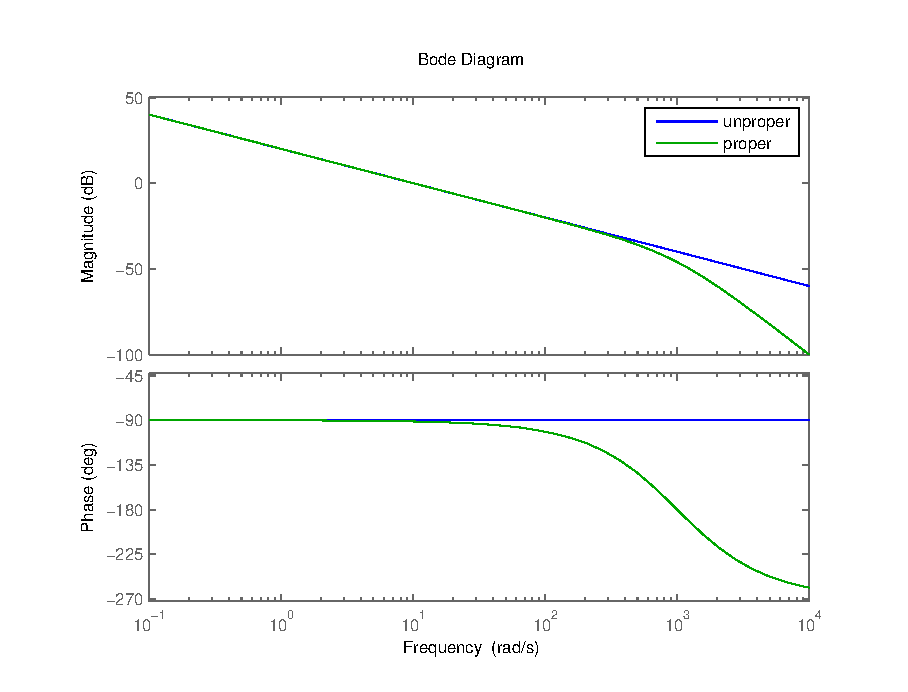
\includegraphics[width=\columnwidth]{fig/bodeProper421.eps}
    \caption{Bode diagram of $L(s)$ with the proper \& unproper $F_y$} 
    \label{bodeProper421}
\end{figure}

\begin{figure}[h!b]
    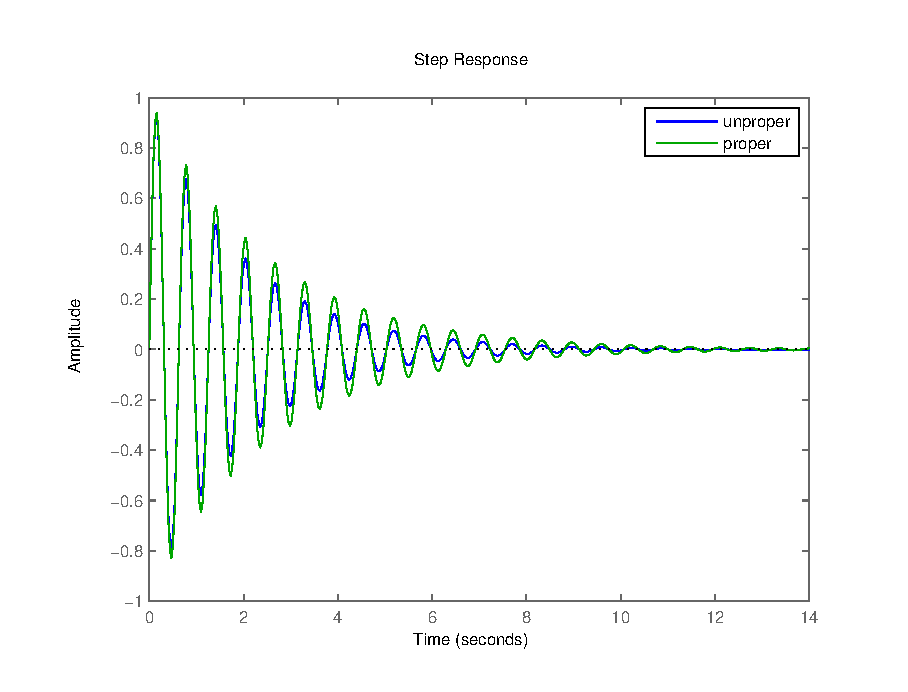
\includegraphics[width=\columnwidth]{fig/stepProper421.eps}
    \caption{Step response of the system with the proper \& unproper $F_y$} 
    \label{bodeProper421}
\end{figure}

